\documentclass{article}
\usepackage[utf8]{inputenc}
\usepackage{amsmath}
\usepackage{tcolorbox}
\usepackage{amssymb}
\usepackage{amsthm}
\usepackage{proof}
\theoremstyle{definition}


\usepackage[
top    = 2.50cm,
bottom = 2.50cm,
left   = 2.75cm,
right  = 2.75cm]{geometry}
\usepackage{fancyhdr}
\pagestyle{fancy}
\lhead{Advanced computation}
\rhead{EPFL/Alp Ozen}
\newcommand{\floor}[1]{\lfloor #1 \rfloor}

\title{Advanced Computation}
\author{alp.ozen}
\date{\vspace{-5ex}}
\newtheorem{theorem}{Theorem}[section]
\newtheorem{example}{Example}
\newtheorem{definition}{Definition}
\newtheorem{question}{Question \textit{???}}
\begin{document}

\maketitle
\section{Propositional logic }
\subsection{Propositions}
A proposition is a declarative sentence that is either true or false. 
\begin{tcolorbox}
How much does it cost? \textbf{is not a proposition}
\\
I like red \textbf{is a proposition}
\end{tcolorbox}

To make life easier, we represent propositional statements through letters such as $p$. 
\\

The conditional statement $p\implies q$ appears very often. Thus, we have the \textit{converse,contrapositive and inverse} which are:
\\
\textbf{converse}: $q \implies p$
\\
\textbf{contrapositive}: $ \neg q \implies \neg p $
\\
\textbf{inverse}: $ \neg p \implies \neg q$
\\

We note that a conditional is logically equivalent to its contrapositive. 

\begin{tcolorbox}
\centering
\begin{array}{cccccc}
 p & q & p $\implies$ q & \neg q & \neg p & \neg q $\implies$ \neg p \\
 \hline
t & t & t & f & f & t\\
t & f & f & t & f & f\\
f & t & t & f & t & t\\
f & f & t & t & t & t
\end{array}
\end{tcolorbox}

\subsection{Precedence of logical operators}

\begin{figure}[h]
    \centering
    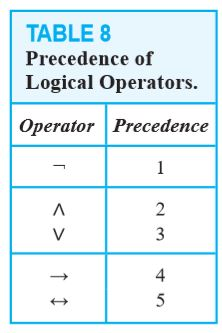
\includegraphics{figures/precedence}
\end{figure}

\subsection{Fuzzy logic}

In fuzzy logic, truth values are between 0 and 1. So if the statement "I like riding a bike" has a value of 0.8, it's negation has 1 minus this value, in this case -0.2. 

\subsection{Applications of logic}
\subsubsection{Logic gates}
Here are the basic logic circuits from which more complex circuits are made: 

\begin{figure}[h]
    \centering
    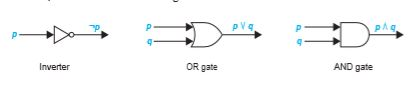
\includegraphics[scale= 1]{epflSemesterOne/advancedComputation/figures/logicgates.JPG}
    \caption{Logic gates}
    \label{fig:my_label}
\end{figure}

Note that the OR and AND gates accept only and only 2 inputs and output one. This input may be as compounded as possible but not exceed 'two chunks'. Thus, when given a complex logical output and reverse engineering, we identify the outer most outer operation, branch it into two or one(if it is simply a negation) and so on. 

\subsubsection{More on propositions}

\begin{tcolorbox}
\begin{itemize}
    \item \textbf{Tautology} is a compound proposition that is always true regardless of the truth value of its variables
    \item \textbf{Contradiction} is a compound proposition that is always false regardless of the truth value of its variables 
    \item \textbf{Contingency} compound statement that is neither tautology nor contradiction
    
    \begin{example}
    \\
    $p \land \neg p$ is a contradiction
    \\
    $p \lor \neg p$ is a tautology
    \end{example}
\end{itemize}
\end{tcolorbox}

Here are some examples of logical calculus:
\\
Show that $\neg(p \lor (\neg p \land q )) \equiveq \neg p \land \neg q$
\begin{align*}
    \neg(p\lor\neg p \land p \lor q)\\
    \neg(T \land p \lor q)\\
    \neg(p \lor q)\\
    \neg p \land \neg q
\end{align*}

\subsubsection{Satisfiability}

A compound proposition is \textbf{satisfiable} if a truth assignment can be made to its variables that make it true making it either a tautology or a contingency. It is \textbf{unsatisfiable} if the negation of the compound statement is a contradiction. 

\subsection{Logical calculus and useful equivalences}

\begin{definition}
If $A \iff B$ is a tautology, then A is logically equivalent to B. 
\end{definition}
\\

Here are some useful logical equivalences(omitting most obvious ones):

\begin{align*}
    p \implies q \equiv \neg p \lor q \equiv \neg(\neg q \lor p) \equiv \neg(q \implies p) \equiv \neg q \implies \neg p \\
    p \lor ( q \land r) \equiv (p \lor q) \land (p \lor r) \\
    \land \ \text{distributes over} \lor \text{and vice versa}\\
    p \lor \neg p \equiv T\\
    p \land \neg p \equiv F\\
    P \land T \equiv p\\
    p \lor F \equiv p
    \ \text{both $\land$ and $\lor$ are associative}
\end{align*}

For more see this figure:

\begin{figure}[h]
    \centering
    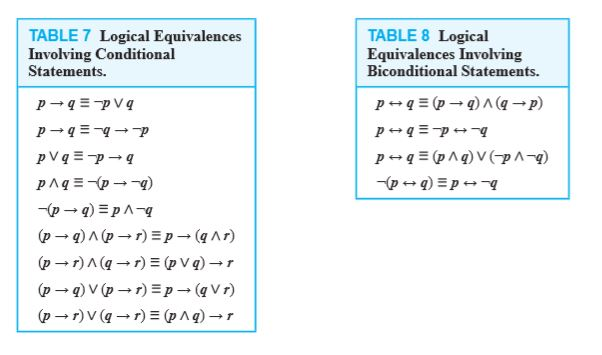
\includegraphics[scale = 0.7]{epflSemesterOne/advancedComputation/figures/logic.JPG}
    \caption{Logic, yey!}
    \label{fig:my_label}
\end{figure}

\begin{definition}
A \textbf{rule of inference} is based on the tautology $p \land (p \implies q) \implies q$. That is, whenever we are given that both $p$ and $p \implies q$ is true, we infer that q must be true. That is :
\\

\infer{q}{p & (p \implies q)}
\end{definition}

Another important fact of logic is that we may boil down all of $\lor, \oplus, \implies, \iff$ to simply propositions involving$\neg, \land$: 

\begin{align*}
    p \lor q \equiv \neg \neg (p \lor q) \equiv \neg(\neg p \land \neg q)\\
    p \oplus q \equiv \neg(p \land q) \land (p \lor q)\\
    p \implies q \equiv \neg p \lor q \equiv \neg (p \land \neg q)\\
    p \iff q \equiv \neg(\neg(p\land q) \land (\neg (\neg p \land \neg q))
\end{align*}


\begin{question}
Given propositional variables and truth values of the single variables for which the compound proposition takes a value, is there a way of deducing a compound proposition? 
\end{question}
\newpage
\subsection{Lec.03 notes}

The \textbf{contrapositive} is the following statement:
\begin{align*}
    p \implies q \equiv \neg p \lor q\\
    \equiv q \lor \neg p\\
    \equiv \neg q \implies \neg p\\
    \therefore p \implies q \equiv \neg q \implies \neg p
\end{align*}
\\
Some useful logical equivalences involving implication:

\begin{align*}
    (p \implies q) \land (p \implies r) \equiv (\neg p \lor q) \land (\neg p \lor r)\\
    \equiv \neg p \lor (q \land r) \equiv p \implies (q \land r)
\end{align*}
And here's a more trivial one: 
\begin{align*}
    (p \implies q) \lor (p \implies r) \equiv (\neg p \lor q) \lor (\neg p \lor r)\\
    \equiv \neg p \lor \neg p \lor q \lor r \equiv \neg p \lor (q \lor r)\\
    \equiv p \implies (q \lor r)
\end{align*}
And slightly more complicated involving De Morgan:
\begin{align*}
    (p \implies r) \land (q \implies r) \equiv (\neg p \lor r) \land (\neg q \lor r)\\
    \equiv \neg r \lor (\neg p \land \neg q) \equiv \neg r \lor (\neg(p \lor q)\\
    \equiv (p \lor q) \implies r 
\end{align*}

We must also add some comments on base b systems of numbers and a general algorithm for conversion. Let's take an example in base 5. Suppose we want to convert $60_{10}$ to its base 5 representation. Well the largest power of 5 less than or equal to 60 is 25 and thus we know that 60 can be \textbf{uniquely} represented as a linear combination of the powers of 5 less than or equal to it. In fact, using powers of 5 less than or equal to 60, we may represent all numbers up to $5^k - 1$ as $4\cdot5^{k-1} + \ldots + 4\cdot5^{0}$. Thus, to represent some $l$ in base $b$ the algorithm is to find the largest power of $b^k < l$, perform $\floor{\frac{l}{b^k}}$ then repeat step 1 and proceed as $l - b^k\cdot\floor{\frac{l}{b^k}}$ and repeat until $l - b^i\cdot\floor{\frac{l}{b^i}} = 0$
 
\subsection{Lec.04 notes}
\subsubsection{More on CMOS}
This was a lecture with a steep curve and here is a summary. First of all, we first revisit some of the concepts of the pmos and nmos resistors. A very important convention is that pmos must never be used for pull-down(connected to GND) and nmos never used for pullup(connected to VDD). 

\begin{figure}[h]
    \centering
    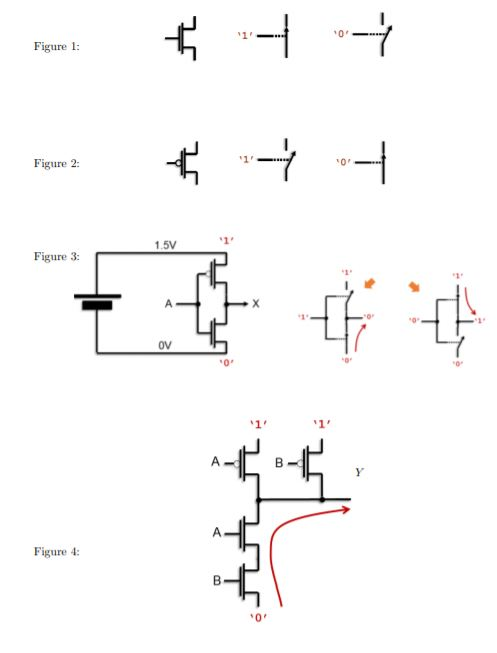
\includegraphics[scale=0.7]{epflSemesterOne/advancedComputation/figures/cmos.JPG}
    \caption{Caption}
    \label{Nmos,Pmos,Inverter,Nand}
\end{figure}

\begin{tcolorbox}
Some principles of cmos gates: 
\begin{itemize}
    \item Pmos goes to top, nmos to bottom.
    \item Never connect high voltage to low voltage to prevent a short circuit. 
    \item Any circuit may be realized as a combination of the NAND and NOR ciruit. 
    \item Each pmos must connect to an nmos. 
\end{itemize}
\end{tcolorbox}
\\
The most challenging part of CMOS circuits is the circuit analysis itself. Consider this example to see a method of circuit analysis: 


\begin{figure}[h!]
    \centering
    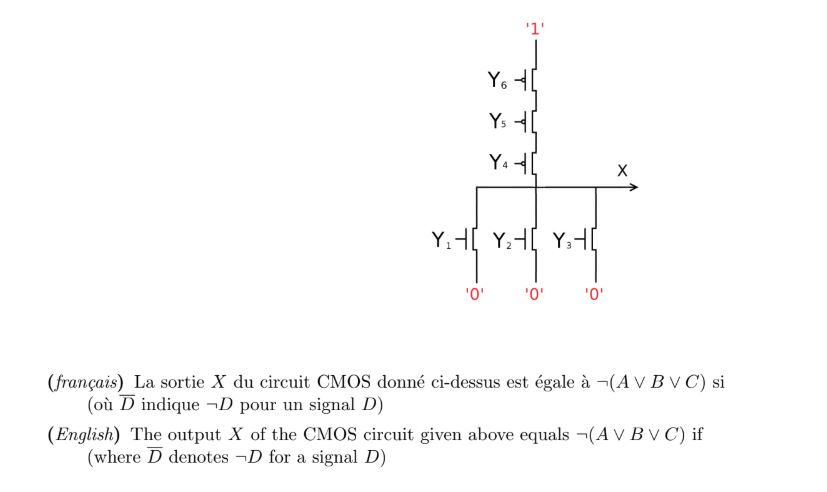
\includegraphics[scale = 0.6]{epflSemesterOne/advancedComputation/figures/cmosq.JPG}
    \caption{exam question}
    \label{exam question}
\end{figure}

\FloatBarrier

\begin{tcolorbox}
Now, first of all, realize that X is connected to VDD iff all of $Y_{6} \land Y_{5} \land Y_{4}$ are grounded. That is $Y_{6} \land Y_{5} \land Y_{4} = 0$. For symbolic purposes, supposing that $Y_{i} = 0 \equiv \neg Y_{i} $ we get that $X = 1 \iff \neg (Y_{4} \lor Y_{5} \lor Y_{6})$ Now given that this is a CMOS circuit, we know that the bottom part does the exact opposite of the upper part. Thus, we have that $X=0 \iff \neg(\neg (Y_{4} \lor Y_{5} \lor Y_{6})) = Y_{4} \lor Y_{5} \lor Y_{6} \equiv Y_{1} \lor Y_{2} \lor Y_{3}$. As a final step, for $\neg (A \lor B \lor C)$ to be true, we need that the output equals $\neg(A \lor B \lor C)$ and since $X=1 \iff \neg (Y_{4} \lor Y_{5} \lor Y_{6})$ we get that $Y_{1} = Y_{2} \ldots$

\end{tcolorbox}

\subsubsection{Binary addition circuit}

Given that we can construct any compound logical gate using CMOS, suppose we want to implement a binary addition calculator. Now here are all the possible cases for doing binary addition: 

\begin{figure}[h]
    \centering
    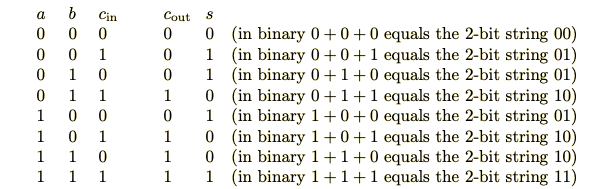
\includegraphics[scale = 0.6]{epflSemesterOne/advancedComputation/figures/binary.png}
    \caption{Addition possibilities}
    \label{fig:my_label}
\end{figure}

Now suppose we want a function $f(a,b,c_{in})$ to evaluate $s$. Well notice that $s$ is only true when the parity of $a,b,c_{in}$ is odd. That is, we may describe this outcome with the function $a \oplus b \oplus c_{in}$. Similarly, devising $g(a,b,c_{in})$ to compute $c_{out}$ we notice that $c_{out}$ evaluates to 1 iff at least two variables are true. This is equivalent to $(a\land b) \lor (a \land c_{in}) \lor (b \land c_{in})$

\subsubsection{Fast Multiplication aka. Karatsuba}
We now ponder whether there is a quick way of multiplying some $v$ and $w$. Now notice that for $v$ and $w$ in base 10, $v = aX + b$ and $w = cX + d$. Now notice that $v \cdot w = (aX+b)(cX+d)$ which in turn is:

\begin{equation*}
    v\cdot w = acX^2 + (ad + bc)X + bd
\end{equation*}

And further notice that:

\begin{equation*}
    ad + bc = (ac + bd) - (a - b)(c - d) 
\end{equation*}

to get:

\begin{equation*}
    v\cdot w = acX^2 + ((ac + bd) - (a - b)(c - d))X + bd
\end{equation*}

Now if for instance $v$ and $w$ were 2 digit numbers, we would normally perform 4 digit by digit multiplications but with this new method, we end up performing only 3 and a trivial subs traction. 
\\
As a general result, for multiplication of two k by k digit numbers, we end up performing $3^{\log_{2}k}$ multiplications and $log_{2}k$ many additions. Finally, notice that Karatsuba is a recursive algorithm. 
\subsubsection{Two's compliment}
Consider how a computer is to represent negative integers. A very smart way of doing so is \textbf{two's compliment}. That is given a binary representation, we invert all 1's with 0's and all 0's with 1's and then add 1. Note that now the 0's take the role of 1's and vice versa. The reason for adding 1 is that the most significant digit is reserved for the sign. A 1 is a negative, a 0 a positive.  



\end{document}